\bibliographyunit[\chapter]

\renewcommand{\chaptermark}[1]{\markboth{#1}{}} 
\chapter*{\mdseries 粮食安全对早期肺功能异常的影响}

\addcontentsline{toc}{chapter}{临床研究}
\markboth{临床研究}{}

\newcommand{\chineseHead}[1]{{\heiti #1}}
\newcommand{\englishTitle}[1]{{\sffamily\centering\Large #1\par}}

% \vspace{24pt}
% \chineseTitle{粮食安全对早期肺功能异常的影响}
% \vspace{24pt} % Space before abstract

% Chinese abstract
\noindent\chineseHead{【摘要】}
黑体,小四号字,左右实心凸形括号。摘要内容书写,宋体, 小四号,两端对齐,字符间距为 常规(标准) 。行距为固定值20磅,段前空0磅, 段后空0磅。
\\ \hspace*{\fill} \\
\noindent\chineseHead{【关键词】}
慢阻肺病;粮食安全;背景保留比值受损肺功能

\vspace{18pt} % Space after Chinese part

\englishTitle{Food insecurity affects PRISm in NHANES}
\vspace{24pt} % Space before abstract

\noindent\textbf{Abstract:} COPD is a xxx
\\ \hspace*{\fill} \\
\noindent\textbf{Keywords:} food insecurity, PRISm, NHANES
English abstract


\renewcommand{\thesection}{\arabic{section}}
\setcounter{section}{0}
\newpage
\section{Introduction}

COPD is a prevalent disease

\section{Method}

Molecular pathology is the expression of a few essential genes which determine disease behavior - e.g., in BC, being hormone receptors (ER, PR, HER2); and Ki67 as proliferation indicator, the expression of which are easily assessed by IHC or IF (immunofluorescence). Positivity is defined differently for each marker - e.g., >=1\% of stained tumor cells for ER or PR while >10\% positive cells for HER2 \citep{fragomeni2018molecular}. ER is a transcription factor (TF) canonically activated by estrogen and is one most essential indicator of endocrine therapy benefits. PR is also a steroid hormone receptor and TF, which can be induced by estrogen and in turn influence ER. Positivity in both ER and PR indicates good prognosis and endocrine responsiveness pathways \citep{lange2008challenges}. HER2 is a receptor tyrosine kinase (RTK) encoded by ERBB2 gene, which when activated, promotes survival, proliferation and invasiveness through activating the PI3K-Akt and Sos-Ras-MAPK pathways \citep{hudis2007trastuzumab}. ERBB2 amplification is detected in 15-30\% of breast cancers, and typically indicates high invasiveness. Anti-HER2 treatment is often suggested - trastuzumab, pertuzumab as monoclonal antibodies (mAb), and small molecules (gefitinib, lapatinib) targeting tyrosine kinase. Ki67 is expressed in active cell cycle, which generally reflects active proliferation and predicts poor outcomes. Chemotherapy is often suggested for tumors with high Ki67 level.


\section{Results}

We found... \citep{adams2019current}

\begin{figure}
    \centering
    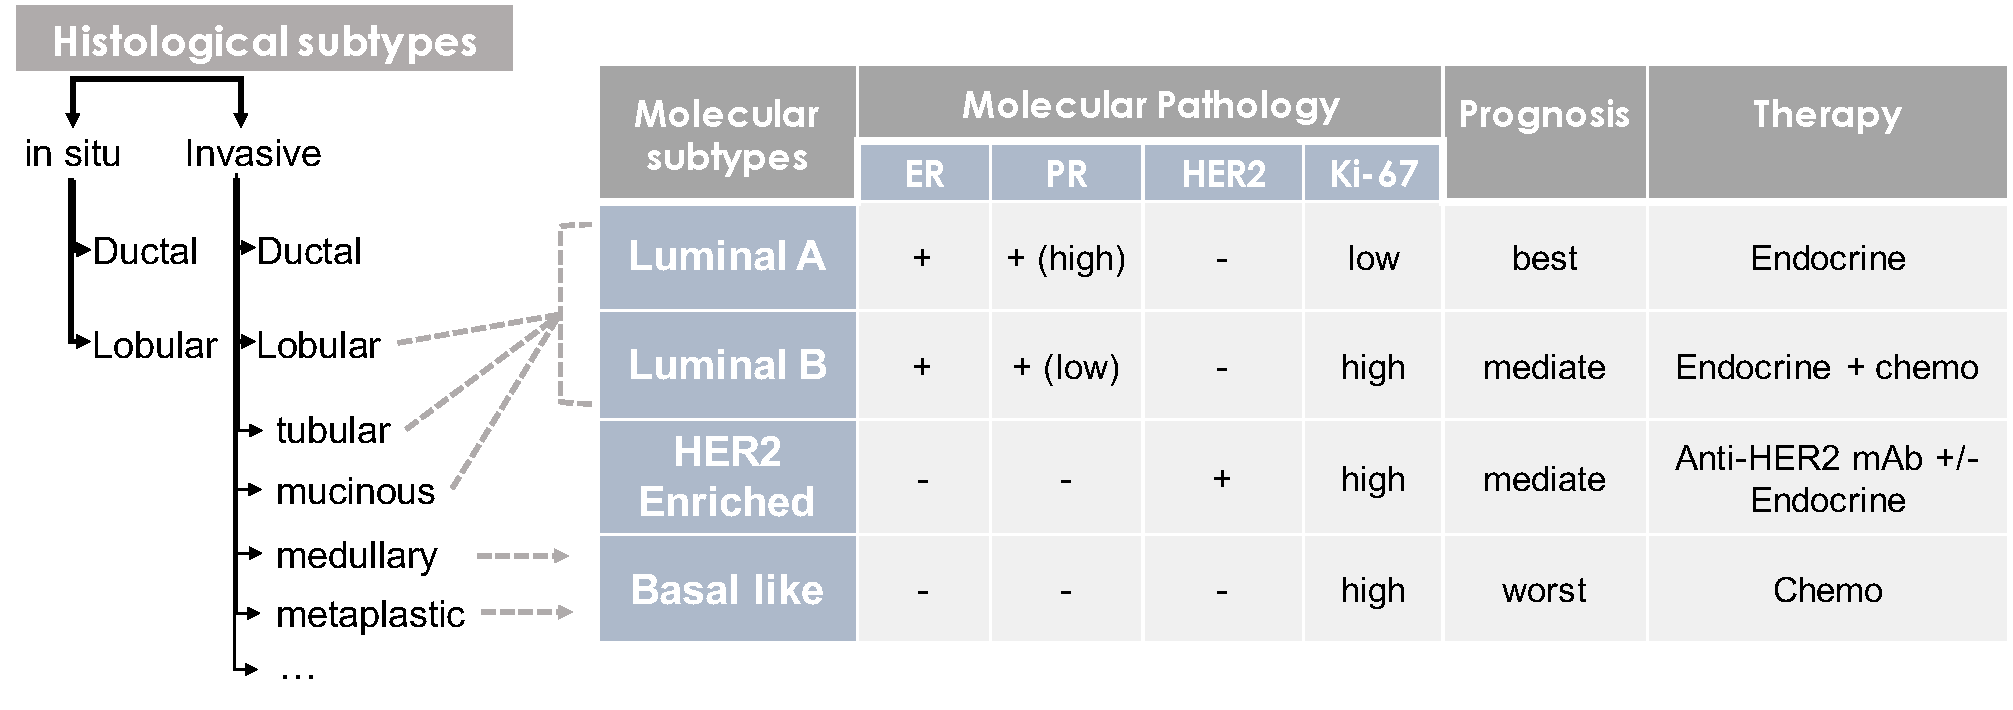
\includegraphics[width=1\linewidth]{intro.subtypes.pdf}
    \caption{Subtypes and therapeutics of breast cancer}
    \caption*{The three major subtyping systems of breast cancer, their relations with prognosis or therapy. ER: estrogen receptor, PR: progesterone receptor, HER2: human epidermal growth factor receptor 2.}
    \label{fig:example}
  \end{figure}

\section{Discussion}

In this research \citep{acar2020exploiting}

Molecular pathology is the expression of a few essential genes which determine disease behavior - e.g., in BC, being hormone receptors (ER, PR, HER2); and Ki67 as proliferation indicator, the expression of which are easily assessed by IHC or IF (immunofluorescence). Positivity is defined differently for each marker - e.g., >=1\% of stained tumor cells for ER or PR while >10\% positive cells for HER2 \citep{fragomeni2018molecular}. ER is a transcription factor (TF) canonically activated by estrogen and is one most essential indicator of endocrine therapy benefits. PR is also a steroid hormone receptor and TF, which can be induced by estrogen and in turn influence ER. Positivity in both ER and PR indicates good prognosis and endocrine responsiveness pathways \citep{lange2008challenges}. HER2 is a receptor tyrosine kinase (RTK) encoded by ERBB2 gene, which when activated, promotes survival, proliferation and invasiveness through activating the PI3K-Akt and Sos-Ras-MAPK pathways \citep{hudis2007trastuzumab}. ERBB2 amplification is detected in 15-30\% of breast cancers, and typically indicates high invasiveness. Anti-HER2 treatment is often suggested - trastuzumab, pertuzumab as monoclonal antibodies (mAb), and small molecules (gefitinib, lapatinib) targeting tyrosine kinase. Ki67 is expressed in active cell cycle, which generally reflects active proliferation and predicts poor outcomes. Chemotherapy is often suggested for tumors with high Ki67 level.

\section*{参考文献}
{\renewcommand{\bibsection}{}
\putbib
}
